
\chapter[Referencial Teórico]{Referencial Teórico}

\section{Câncer de pele}

    ``O câncer de pele é provocado pelo crescimento anormal e descontrolado das células que compõem a pele. Essas células se dispõem formando camadas e, de acordo com as que forem afetadas, são definidos os diferentes tipos de câncer''\cite{sbd}.
    
    Existem dois tipos de cânceres de pele, o melanoma e os carcinomas. O melanoma é o tipo mais agressivo, mas seus casos são relativamente raros. Já os carcinomas tem letalidade baixa, mas  o número de casos é extremamente alto no Brasil.
    
    Geralmente, o cancêr de pele é o menos agressivo dentre os outros cânceres existentes, mas se houver um diagnóstico tardio, este pode levar a ferimentos, sérias deformidades físicas e até a morte.
    
               
    O Instituto Nacional do Cancêr (INCA) afirma que  \begin{quotation}
    
    
    
    ``Estima-se que no Brasil existem 85.170 casos recentes de câncer de pele não melanoma entre homens e 80.410 nas mulheres para cada ano do biênio 2018-2019. Esses valores correspondem a um risco estimado de 82,53 casos novos a cada 100 mil homens e 75,84 para cada 100 mil mulheres''\cite[p.54]{Estimativa}.
  \end{quotation}
    .%http://www.inca.gov.br/estimativa/2018/sintese-de-resultados-comentarios.asp
              
    Em seu estudo a Sociedade Brasileira de Dermatologia diz que  o maior motivo para evolução do cancêr de pele é devido a exposição aos raios ultravioletas irradiados pelo sol. Os horários mais perigosos são no período de 10 às 16 horas. Evitar a exposição intensa ao sol nesses horários e proteger a pele dos impactos da radiação ultravioleta são os melhores métodos para evitar os tumores de pele.%http://www.sbd.org.br/

 


 Há várias formas de tratamento atualmente, mas todos os casos precisam ser identificados antecipadamente para melhores chances de cura. Uma forma de realizar tal feito  é detectar tumores através da temperatura da pele, utilizando-se de equipamentos médicos.
 
 Em sua teste  Fabrício \cite{Fabricio} alega que diferentemente da trombose ou esclerose vascular que reduz o sangue  fluído na pele e consequentemente diminui a temperatura superficial da mesma, os tumores de pele provocam um aumento de temperatura local, por essa razão a temperatura incomum da pele pode apontar circulação sanguínea irregular.
 Lawson\cite{Lawson} consolida esse fato afirmando que  sangue venoso que escoa o tumor maligno é regularmente mais quente  do que o fornecido pelo sistema arterial . Ele também menciona que foi realizada uma experiência com 26 pacientes portadores de câncer de mama que comprovou que a temperatura da pele sobre o tumor na mama era maior que a do tecido normal. 
    
\begin{quotation}
 O aumento médio de temperatura detectável na área do tumor foi de $ 2.27^{\circ}F$ . O máximo foi de $ 3.5^{\circ}F $ e o mínimo de $ 1.3^{\circ}F$ . Em dois casos adicionais mostrando um aumento entre $ 1.5^{\circ} $  e $ 2^{\circ}F$ , o diagnóstico foi de malignidade duvidosa\cite[p.309]{Lawson}.\end{quotation}%CLINICAL AND LABORATORY NOTES- IMPLICATIONS OF SURFACE TEMPERATURES IN THE DIAGNOSIS OF BREAST CANCER- RAY LAWSON, M.D, MONTREAL - CANAD, M.A.J AUG.15,1956.VOL.75 --- https://www.ncbi.nlm.nih.gov/pmc/articles/PMC1824571/?page=1
 
   %CLINICAL AND LABORATORY NOTES- IMPLICATIONS OF SURFACE TEMPERATURES IN THE DIAGNOSIS OF BREAST CANCER- RAY LAWSON, M.D, MONTREAL - CANAD, M.A.J AUG.15,1956.VOL.75------https://www.ncbi.nlm.nih.gov/pmc/articles/PMC1824571/?page=1


   
   
   %ANÁLISE INVERSA COM USO DE ALGORITMO GENÉTICO PARA LOCALIZAÇÃO DE TUMORES DE PELE DISCRETIZADOS EM ELEMENTOS DE CONTORNO COM RECIPROCIDADE DUAL - FABRÍCIO RIBEIRO BUENO-DISSERTAÇÃO DE MESTRADO EM ESTRUTURAS E CONSTRUÇÃO CIVIL- DEPARTAMENTO DE ENGENHARIA CIVIL E AMBIENTAL - BRASÍLIA/DF AGOSTO DE 2008}
  
   Lawson afirma que:\begin{quotation} 
  
  ``As propensões malignas são diretamente relacionadas à velocidade de divisão celular. Esta por sua vez é refletida pelo metabolismo local acelerado que é adequadamente apoiada pelo aumento da vascularização sanguínea e linfática. Essas biológicas alterações podem ser prontamente detectadas estimando mudanças de temperatura no tumor ou seu ambiente imediato. A energia térmica é transferida pelo processo de convecção, condução e radiação''\cite[p.309]{Lawson} .\end{quotation}
%CLINICAL AND LABORATORY NOTES- IMPLICATIONS OF SURFACE TEMPERATURES IN THE DIAGNOSIS OF BREAST CANCER- RAY LAWSON, M.D, MONTREAL - CANAD, M.A.J AUG.15,1956.VOL.75%
  
 Logo, tal fato pode ser utilizado para disgnósticos de tumores em tecidos vivos.
 %CLINICAL AND LABORATORY NOTES- IMPLICATIONS OF SURFACE TEMPERATURES IN THE DIAGNOSIS OF BREAST CANCER- RAY LAWSON, M.D, MONTREAL - CANAD, M.A.J AUG.15,1956.VOL.75
   

   
  
  Ao longo dos anos foram utilizados alguns métodos para medir essa  temperatura corporal, como por exemplo o primeiro experimento de Pennes, em 1948, que com intuito de medir a temperatura do antebraço  foi utilizado uma agulha de aço inoxidável para a introdução de um termopar(sensor utilizado para medição de temperatura).
 
 \begin{figure}[h]
\centering
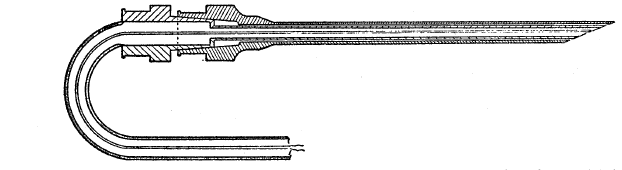
\includegraphics[width=10cm]{figuras/agulha.png}
\caption{Agulha de aço inoxidável usada para introdução de termopar. FONTE: \cite{PENNES}}.
\label{figura 1:Agulha }
\end{figure}

De acordo com \cite{Lawson}, o termopar também foi usado em outras experiências, mas sem o uso de agulhas, a técnica simplismente se resumia a aplicar o termopar  na pele sobre o tumor, ou, no caso de uma neoplasia (massa anormal de tecido) profundamente enraizada, na aréola ipsilateral (pequena área circular que envolve o mamilo). Se o paciente portasse o câncer, haveria um diferencial de temperatura.
 
 
 \begin{figure}[h]
\centering
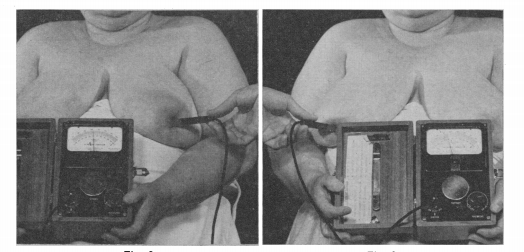
\includegraphics[width=10cm]{figuras/termopar_na_mama.png}
\caption{Carcinoma de mama esquerda.Mama direita negativa no mesmo paciente, mostrando
diferencial de temperatura. FONTE: \cite{Lawson}}.
\label{figura 2 :termopar na mama}
\end{figure}

   Outro método empregue foi o uso do Evaporógrafo Baird,  um instrumento projetado para dar uma imagem térmica direta em um filme de óleo muito fino. ``O princípio principal empregado neste aparelho é a evaporação diferencial de um filme de óleo em uma membrana transparente que
pode ser observado ou fotografado em preto e
branco ou colorido'' \cite{Lawson}. O equipamento dispõe-se de uma alta resolução em locais onde a temperatura é maior e má resolução onde a temperatura é menor.

\begin{figure}[h]
\centering
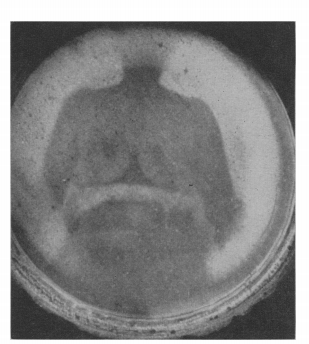
\includegraphics[width=8cm]{figuras/Evaporografo.png}
\caption{-Evaporógrafo de paciente com carcinoma
de mama direita. FONTE: \cite{Lawson}}.
\label{figura 3:Evaporógrafo}
\end{figure}

 Atualmente detemos de técnicas e equipamentos mais modernos.  
Como já foi dito, a definição da temperatura em tecidos se dá por intermédio da transferência de calor nos mesmos e utilizando a ``equação biotérmica de Pennes é possível encontrar a distruibuição de temperatura e o fluxo de calor em um maciço de pele''\cite{Fabricio}. %ANÁLISE INVERSA COM USO DE ALGORITMO GENÉTICO PARA LOCALIZAÇÃO DE TUMORES DE PELE DISCRETIZADOS EM ELEMENTOS DE CONTORNO COM RECIPROCIDADE DUAL - FABRÍCIO RIBEIRO BUENO-DISSERTAÇÃO DE MESTRADO EM ESTRUTURAS E CONSTRUÇÃO CIVIL- DEPARTAMENTO DE ENGENHARIA CIVIL E AMBIENTAL - BRASÍLIA/DF AGOSTO DE 2008}






\section{Harry H. Pennes e a Equação da Biotransferência de calor}

     Pennes, em 1948, `` foi o primeiro a propor um modelo matemático que representasse o processo de biotransferência de calor''\cite[p.28]{Marcus}.
     Realizou-se experimentos afim de estudar a difusão de calor no corpo humano.
      
       % %INSTITUTO MILITAR DE ENGENHARIA - MARCUS VINICIUS COSTA DE SOUZA- OTIMIZAÇÃO DE TERMOS FONTES EM PROBLEMAS DE %BIOTRANSFERÊNCIA DE CALOR- RIO DE JANEIRO-2009
      \begin{quotation}
     ``As temperaturas dos tecidos normais do antebraço humano e do sangue arterial braquial foram medidas para avaliar a aplicabilidade da teoria do fluxo de calor ao antebraço em termos básicos de taxa local de produção de calor tecidual e fluxo volumétrico de sangue ''\cite{PENNES}. \end{quotation}

   %\emph{   ANALYSIS OF TISSUE AND ARTERIAL BLOOD TEMPERATURES IN THE RESTING HUMAN FOREARM - AUGUST 1948- NEW YORK- HARRY %H.PENNES}
   Com esse contéudo elaborou-se uma equação que descreve a propagação de calor no corpo humano, denominada de Equação da Biotransferência de Calor ( Bioheat Transfer Equation - BHTE).


      De acordo com \apud{PENNES}{Olho}
 \begin{quotation} ``A transferência de calor nos organismos vivos é caracterizada por dois mecanismos importantes: metabolismo e fluxo sanguíneo. O sangue escoa, de forma não-newtoniana, através dos vasos sanguíneos que apresentam diferentes dimensões. Segundo a teoria de Pennes, a transferência líquida de calor entre o sangue e o tecido é proporcional à diferença entre a temperatura do sangue arterial, que entra no tecido, e a temperatura do sangue venoso que sai do tecido. Ele sugeriu que a transferência de calor devida ao escoamento sanguíneo pode ser modelada por uma taxa de perfusão sanguínea, com o sangue atuando como uma fonte/sumidouro escalar de calor. Apesar da sua simplicidade, uma das dificuldades encontradas no uso da BHTE reside na ausência de informação detalhada e precisa sobre as taxas volumétricas de perfusão sanguínea, especialmente para tecidos neoplásico''\cite{Olho}.\end{quotation}
       %
      %http://www.scielo.br  - Revista brasileira de Engenharia Biomédica  Rev. Bras. Eng. Bioméd. vol.29 no.1 Rio de Janeiro %Jan./Mar. 2013 - Análise computacional do dano térmico no olho humano portador de um melanoma de coroide quando submetido à %termoterapia transpupilar a laser - José Duarte da SilvaI,*; Paulo Roberto Maciel LyraII; Rita de Cássia Fernandes de %LimaII
     % IInstituto Federal de Educação, Ciência e Tecnologia de Pernambuco – IFPE, Av. Professor Luiz Freire, 500, Cidade %Universitária, CEP 50740-540, Recife, PE, Brasil
      %IIDepartamento de Engenharia Mecânica, Universidade Federal de Pernambuco – UFPE, Av. Acadêmico Hélio Ramos, s/n, Cidade %Universitária, CEP 50740-530, Recife, PE, Brasil

      Houve vários estudos com o objetivo de aperfeiçoar a equação de biotransferência de calor de Pennes, porém, acabaram em modelos muito específicos e complexos. Por esses motivos e por sua clareza, a equação de Pennes ainda é a mais usada para caracterizar a transferência de calor e a disseminação da temperatura em tecidos biológicos vivos.




 \subsection{Modelo físico-matemático}

    Segundo \cite{Carla}, a equação abaixo descreve a transferência de calor nos organismos vivos e é chamada de Equação de Pennes. 
   %MODELAGEM COMPUTACIONAL DA BIOTRANSFERÊNCIA  DE CALOR NO  TRATAMENTO  POR HIPERTERMIA EM TUMORES DE DUODENO ATRAVÉS DO MÉTODO DOS VOLUMES FINITOS  EM MALHAS  NÃO-ESTRUTURADAS- UNIVERSIDADE FEDERAL DE PERNAMBUCO-CURSO DE PÓS-GRADUAÇÃO EM ENGENHARIA MECÂNICA-CARLA SIMONE CARDOSO GUIMARÃES , RECIFE, FEVEREIRO DE 2003;
   

  \begin{equation}\rho c\frac{\partial T}{\partial t} = K_{t}\nabla^{2}T+ Q_{p} + Q_{m} + Q . \end{equation}


  onde:


 $ K_{t} $ = Condutividade térmica do tecido $[W/m^{\circ}C];$ 

  $\rho $= Massa específica do tecido $[kg/m^3];$

 c = Calor específico do tecido $[J/kg^{\circ}C];$

  T = Temperatura $[^{\circ}C];$

  t = Tempo [s];

   $ Q_{p} $= Fonte de calor devido à perfusão sanguínea $[W/m^3];$


   $Q_{m} $= Fonte de calor devido à geração de calor metábolico $[W/m^3];$

  Q = Fonte externa de calor sobre o domínio $[W/m^3];$

 O termo {\itshape Q} pode ser qualquer fonte de aquecimento externa, como sementes ferromagnéticas e radiação eletromagnética, como radiofrequência, microondas, ultra-som, e laser \cite[p.10]{Giselle}. Já o termo {\itshape $Q_{m}$}, conforme o estudo de  Sturesson \& Andersson-Engels, ``A  fonte de calor devido à geração metábolica é normalmente muito menor do que o calor externo depositado, então este termo pode ser desconsiderado da expressão'' \apud[p.2039]{Jain}{Andersson}. %UNIVERSIDADE FEDERAL DE PERNAMBUCO- CURSO DE PÓS -GRADUAÇÃO EM ENGENHARIA MEC NICA - ANÁLISE DA BIOTRANSFERÊNCIA DE CALOR  NOS TECIDOS OCULARES DEVIDO À PRESENÇA DE IMPLANTES RETINIANOS ATRAVÉS DA UTILIZAÇÃO DO MÉTODO DOS VOLUMES FINITOS EM MALHAS NÃO-ESTRUTURADAS AUTOR: GISELLE MARIA LOPES LEITE DA SILVA, RECIFE, MARÇO DE 2004. Já o termo Qm,conforme o estudo de  Sturesson & Andersson-Engels(1995,p.2039 apud Jain ,1983,p.9-46), a  fonte de calor devido à geração metábolica é normalmente muito menor do que o calor externo depositado, então este termo pode ser desconsiderado da expressão.%Jain R K 1983 Bioheat transfer: mathematical models of thermal systems Hyperthermia in Cancer Therapy ed F K Storm  Boston: HAll) pp 9-46.

       ``O termo {\itshape $Q_{p}$} corresponde a fonte de calor devido à perfusão sanguínea que caracteriza-se pela transferência de calor efetuada pelo sangue através da vascularização capilar presente nos tecidos vivos'' \cite{Carla}.%CARLA SIMONE CARDOSO GUIMARÃES - MODELAGEM COMPUTACIONAL DA BIOTRANSFERÊNCIA DE CALOR NO  TRATAMENTO POR HIPERTERMIA EM TURMORES DE DUODENO ATRAVÉS DO MÉTODO  DOS VOLUMES FINITOS EM MALHAS NÃO-ESTRUTURADAS- UNIVERSIDADE FEDERAL DE PERNAMBUCO- CURSO DE PÓS-GRADUAÇÃO EM ENGNEHARIA MECÂNICA- RECIFE, FEVEREIRO DE 2003. % 
       De acordo com \cite{Giselle},  {\itshape $Q_{p}$} é dado pela equação abaixo:


    \begin{equation} Q_{p}= \omega\times\rho_{s}\times c_{s}\times\rho\times(Ta-Tv).\end{equation} 

       Onde:

       $\omega$ = Taxa de perfusão sanguínea $[m^3 de sangue/m^3 de tecido.s];$

      $ \rho_{s} $= Massa específica do sangue $[kg/m^3];$

        $c_{s} $= Calor específico do sangue  $[J/kg.^{\circ}C]$

        $T_{a}$ = Temperatura arterial do sangue entrando no tecido$ [^{\circ}C];$

      $T_{v}$ = Temperatura do sangue venoso saindo do tecido $[^{\circ}C];$









%UNIVERSIDADE FEDERAL DE PERNAMBUCO- CURSO DE PÓS -GRADUAÇÃO EM ENGENHARIA MEC NICA - ANÁLISE DA BIOTRANSFERÊNCIA DE CALOR  NOS TECIDOS OCULARES DEVIDO À PRESENÇA DE IMPLANTES RETINIANOS ATRAVÉS DA UTILIZAÇÃO DO MÉTODO DOS VOLUMES FINITOS EM MALHAS NÃO-ESTRUTURADAS AUTOR: GISELLE MARIA LOPES LEITE DA SILVA, RECIFE, MARÇO DE 2004

  Reescrevendo a Eq.(1.1) em coordenadas cartesianas e desconsiderando o termo de geração de calor metábolico pelo motivo já explicado antes, temos:



  \begin{equation}\rho c\frac{\partial T}{\partial t} = \frac{\partial }{\partial x} \left (K_{t}\frac{\partial T}{\partial x}\right ) + \frac{\partial }{\partial y} \left(K_{t}\frac{\partial T}{\partial y}\right ) + \frac{\partial }{\partial z} \left (K_{t}\frac{\partial T}{\partial z}\right ) + Q_{p} + Q.\end{equation}
  
   A dificuldade dessa equação diferencial é que ela não pode ser resolvida analiticamente, então é necessário utilizar-se de algum método númerico para se obter uma aproximação do resultado.
   
   Os métodos númericos mais utilizados para resolver esse tipo de equação é o Método das Diferenças Finitas (MDF), Método dos Elementos Finitos (MEF), Método dos Volumes Finitos (MVF), e o Método dos Elementos de Contorno (MEC);
   
   O objetivo deste trabalho é alcançar essa solução  utilizando um método diferente, o Método da Decomposição de Adomian.
  
  
%UNIVERSIDADE FEDERAL DE PERNAMBUCO- CURSO DE PÓS -GRADUAÇÃO EM ENGENHARIA MEC NICA - ANÁLISE DA BIOTRANSFERÊNCIA DE CALOR  NOS TECIDOS OCULARES DEVIDO À PRESENÇA DE IMPLANTES RETINIANOS ATRAVÉS DA UTILIZAÇÃO DO MÉTODO DOS VOLUMES FINITOS EM MALHAS NÃO-ESTRUTURADAS AUTOR: GISELLE MARIA LOPES LEITE DA SILVA, RECIFE, MARÇO DE 2004

% AN INVERSE GEOMETRY PROBLEM FOR THE LOCALIZATION OF SKIN TUMOURS BY THERMAL ANALYSIS - P W PARTRIDGE AND L C WROBEL - SCHOOL OF ENGINEERING AND DESIGN, BRUNEL UNIVERSITY, UXBRIDGE, MIDDLESEX UB8 3PH,UK.




          
              